\documentclass{beamer}
\mode<presentation>
%\usetheme{Warsaw}

\usepackage{amsmath, amssymb, amsthm, graphicx, enumerate, subfigure}
\usepackage{verbatim}
\usepackage[spanish,mexico]{babel}
\usepackage[utf8]{inputenc}
\usepackage[labelformat=empty]{caption}
\usepackage{pifont}% http://ctan.org/pkg/pifont

\definecolor{green1}{rgb}{0.1,0.5,0.2}
\definecolor{green2}{rgb}{0.9,1,0.9}
\definecolor{green3}{rgb}{0.1,0.3,0.2}
\definecolor{green4}{rgb}{0.9,1,0.9}

\useinnertheme{rectangles}


\setbeamercolor*{Title bar}{fg=white, bg=green1}
\setbeamercolor*{section in head/foot}{bg=green1,fg=white}
\setbeamercolor*{title}{fg=white, bg=green1}
\setbeamercolor*{Location bar}{fg=white,bg=green}
\setbeamercolor*{frametitle}{parent=Title bar}
\setbeamercolor*{block title}{bg=green1,fg=white}
\setbeamercolor*{block body}{bg=green2,fg=green3}
\setbeamercolor*{normal text}{bg=white,fg=green3}
\setbeamercolor*{structure}{bg=white,fg=green1}

\newtheorem{defn}{Definición}
\newtheorem{teo}{Teorema}
\newtheorem{prop}{Proposición}

\newcommand{\R}{\mathbb{R}}
\newcommand{\cmark}{\ding{51}}
\newcommand{\xmark}{\ding{55}}

\title{Sistema de recomendación de hoteles similares}
\subtitle{TESIS}
\institute{
\includegraphics[width=0.3\textwidth]{imagenes/logo_ITAM.jpg}\\INSTITUTO TECNOLÓGICO AUTÓNOMO DE MÉXICO}
\author{Felipe Gerard Valdés}
\date{Febrero de 2015}



\AtBeginSection[]
{
	\begin{frame}<beamer>{Agenda}
		\tableofcontents[currentsection]
	\end{frame}
}


\begin{document}

%%%%%%%%%%%%%%%%% frame %%%%%%%%%%%%%%%%%%%%%%%%%

\begin{frame}
	\titlepage
\end{frame}

%%%%%%%%%%%%%%%%% frame %%%%%%%%%%%%%%%%%%%%%%%%%
\begin{frame}{Agenda}
	\tableofcontents
\end{frame}

%%%%%%%%%%%%%%%%%%%%%%%%%%%%%%%%%%%%%%%%%%%%%%%%%
\begin{frame}{}
\end{frame}

%%%%%%%%%%%%%%%%%%%%%%%%%%%%%%%%%%%%%%%%%%%%%%%%%
\begin{frame}{}
	\begin{itemize}%[<+->] 
		\item .
	\end{itemize}
\end{frame}

%%%%%%%%%%%%%%%%%%%%%%%%%%%%%%%%%%%%%%%%%%%%%%%%%
%%%%%%%%%%%%%%%%%%%%%%%%%%%%%%%%%%%%%%%%%%%%%%%%%
\section{Planteamiento}

%%%%%%%%%%%%%%%%%%%%%%%%%%%%%%%%%%%%%%%%%%%%%%%%%
\begin{frame}{Antecedentes}
	\begin{itemize}%[<+->]
		\item Las ventas de viajes por Internet no tienen asistencia humana
		\item Muchos clientes no conocen los destinos que planean visitar
		\item No basta con permitir que el cliente explore una lista de hoteles
		\item \textbf{Objetivo:} Facilitar la búsqueda del hotel correcto para incrementar las ventas
		\item[$\mathbf{\rightarrow}$] \textbf{Idea:} Para cada hotel, recomendar una lista de hoteles ``similares''
		\item Situación actual:
		\begin{itemize}
			\item Recomendaciones estáticas
			\item Criterio:
			\begin{itemize}
				\item \textbf{Destino:} Usualmente es una ciudad o zona
				\item \textbf{Estrellas:} Categoría del hotel
			\end{itemize}
		\end{itemize}
		\item No está mal, pero ¿se puede mejorar?
	\end{itemize}
\end{frame}

%%%%%%%%%%%%%%%%%%%%%%%%%%%%%%%%%%%%%%%%%%%%%%%%%
\begin{frame}{Análisis de la competencia}
	\begin{itemize}%[<+->] 
		\item Competidores principales: Price Travel, Booking, Despegar, Expedia. Bonus: Trip Advisor
		\item Diversas formas de recomendar:
		\begin{itemize}
			\item Hoteles recientemente vistos: No son recomendaciones genuinas
			\item Hoteles cercanos / en el mismo destino: Estilo y precios pueden ser muy distintos
			\item Recomendaciones con métodos desconocidos (p.ej. ``a otros usuarios les gustó...''): Calidad variable; en general son demasiado rígidos
		\end{itemize}
	\item \textbf{Conclusión:} La competencia deja mucho que desear, pero hay mucho qué aprender
	\end{itemize}
\end{frame}

%%%%%%%%%%%%%%%%%%%%%%%%%%%%%%%%%%%%%%%%%%%%%%%%%
\begin{frame}{\textit{¿Qué queremos?}}
	\begin{itemize}%[<+->] 
		\item Evitar mostrar hoteles demasiado caros
		\item Tomar en cuenta el perfil del hotel
		\item Incorporar información geográfica más detallada que el destino
		\item Que el criterio se adapte a distintos tipos de zonas
		\item Que no se acaben las recomendaciones nuevas (efecto laberinto)
	\end{itemize}
\end{frame}

%%%%%%%%%%%%%%%%%%%%%%%%%%%%%%%%%%%%%%%%%%%%%%%%%
%%%%%%%%%%%%%%%%%%%%%%%%%%%%%%%%%%%%%%%%%%%%%%%%%
\section{Solución}

%%%%%%%%%%%%%%%%%%%%%%%%%%%%%%%%%%%%%%%%%%%%%%%%%
\begin{frame}{Plan de ataque}
	\begin{enumerate}%[<+->] 
		\item \textbf{Precio:} Filtrar hoteles demasiado caros
		\item \textbf{Similitud:} Construir un \textit{criterio integral de similitud}
		\begin{itemize}
			\item Cantidad de servicios
			\item Perfil similar
		\end{itemize}
		\item \textbf{Distancia:} Recomendar hoteles geográficamente cercanos
	\end{enumerate}
\end{frame}

%%%%%%%%%%%%%%%%%%%%%%%%%%%%%%%%%%%%%%%%%%%%%%%%%
\begin{frame}{Precio}
	\begin{itemize}%[<+->] 
		\item Poner hoteles demasiado caros no promueve el interés del cliente
		\item Generalmente más barato es mejor (siempre y cuando tenga la categoría suficiente)
		\item[$\mathbf{\rightarrow}$] Porcentaje máximo arriba del hotel original
		\item Hoteles por encima del precio establecido son invisibles
	\end{itemize}
\end{frame}

%%%%%%%%%%%%%%%%%%%%%%%%%%%%%%%%%%%%%%%%%%%%%%%%%
\begin{frame}{Similitud (P1)}
	\begin{itemize}%[<+->] 
		\item \textbf{Caracterización}
		\begin{itemize}
			\item No bastan las estrellas
			\item Usar información de servicios
			\item Usarla directamente es ruidoso porque no toma en cuenta sustitutos
			\item \textbf{Solución:} Agrupar los servicios en categorías
			\item \textbf{Método:} Manual (criterio de negocio) + aglomerado jerárquico
		\end{itemize}
	\end{itemize}
\end{frame}

%%%%%%%%%%%%%%%%%%%%%%%%%%%%%%%%%%%%%%%%%%%%%%%%%
\begin{frame}{Similitud (P2)}
	\begin{itemize}%[<+->] 
		\item La similitud se puede dividir en dos aspectos básicos
		\item \textbf{Servicios:}
		\begin{itemize}
			\item Al menos ciertos servicios (~ estrellas)
			\item Los servicios faltantes restan similitud
			\item Los servicios extras no se penalizan
		\end{itemize}
		\item \textbf{Perfil:}
		\begin{itemize}
			\item Hoteles del mismo estilo
			\item Misma proporción de cada categoría
			\item Ignorar la cantidad de servicios
			\item Podría dar hoteles más sencillos o más lujosos
		\end{itemize}
	\end{itemize}
\end{frame}

%%%%%%%%%%%%%%%%%%%%%%%%%%%%%%%%%%%%%%%%%%%%%%%%%
\begin{frame}{Similitud (P2)}
	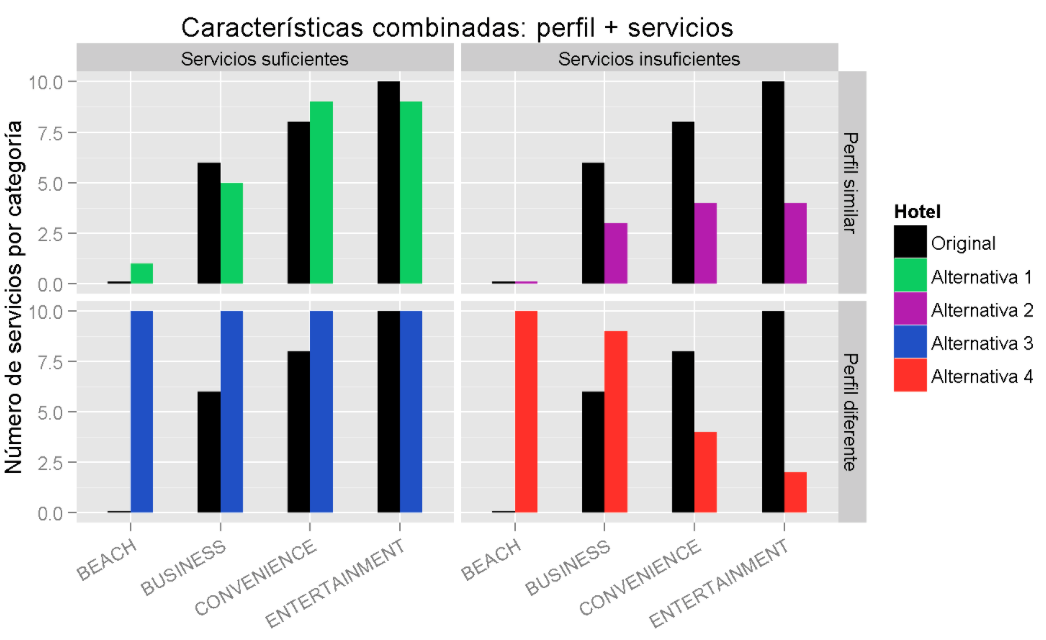
\includegraphics[width=\textwidth]{imagenes/similitud.png}
\end{frame}


%%%%%%%%%%%%%%%%%%%%%%%%%%%%%%%%%%%%%%%%%%%%%%%%%
\begin{frame}{Similitud (P3)}
	\begin{itemize}%[<+->] 
		\item Medida de similitud de servicios: Calidad mínima
		\item Medida de similitud de perfil: Proporciones de servicios
		\item Medida de similitud final:
		\begin{itemize}
			\item Capturar ambos efectos
			\item Promedio ponderado entre ambas medidas
			\item Ponderación de acuerdo a la variabilidad de cada una (PCA)
		\end{itemize}
		\item ¿Por qué no diferencia absoluta?
		\begin{itemize}
			\item Es muy agresiva
			\item No es ajustable
		\end{itemize}
	\end{itemize}
\end{frame}

%%%%%%%%%%%%%%%%%%%%%%%%%%%%%%%%%%%%%%%%%%%%%%%%%
\begin{frame}{Distancia}
	\begin{itemize}%[<+->] 
		\item Hoteles cercanos (usando coordenadas)
		\item El significado de ``cerca'' es variable
		\item Se necesita un criterio dinámico
		\item Cuidar que los hoteles distintos no afecten
	\end{itemize}
\end{frame}

%%%%%%%%%%%%%%%%%%%%%%%%%%%%%%%%%%%%%%%%%%%%%%%%%
\begin{frame}{Distancia}
	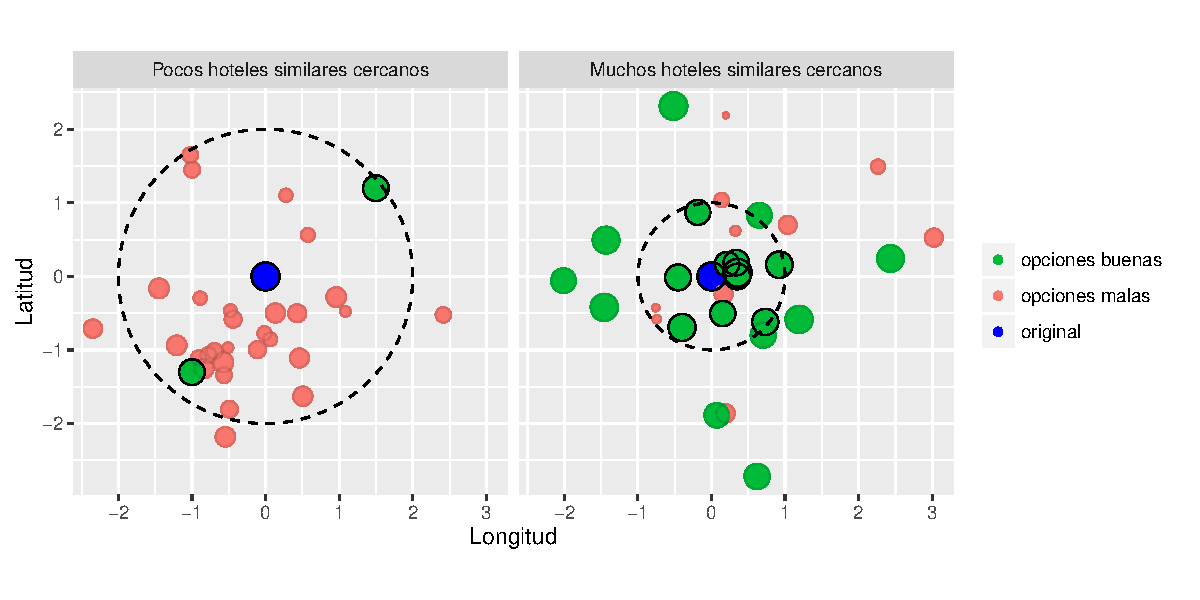
\includegraphics[width=\textwidth]{imagenes/distdin.pdf}
\end{frame}

%%%%%%%%%%%%%%%%%%%%%%%%%%%%%%%%%%%%%%%%%%%%%%%%%
\begin{frame}{Modelo completo}
	\begin{enumerate}%[<+->]
		\item Agrupar los servicios en categorías
		\item Calcular la ponderación entre servicios y perfil
		\item Definir una \textbf{geocerca} (radio de cercanía razonable) alrededor de cada hotel
		\begin{itemize}
			\item Ignorar hoteles caros (precio de largo plazo)
			\item Acumular una cantidad de similitud (mayor peso a hoteles parecidos, menor a los diferentes)
		\end{itemize}
		\item Recomendar dentro de la geocerca de acuerdo a la \textbf{similitud}
	\end{enumerate}
\end{frame}

%%%%%%%%%%%%%%%%%%%%%%%%%%%%%%%%%%%%%%%%%%%%%%%%%
%%%%%%%%%%%%%%%%%%%%%%%%%%%%%%%%%%%%%%%%%%%%%%%%%
\section{Implementación}

%%%%%%%%%%%%%%%%%%%%%%%%%%%%%%%%%%%%%%%%%%%%%%%%%
\begin{frame}{Arquitectura: SQL + \texttt{R}}
	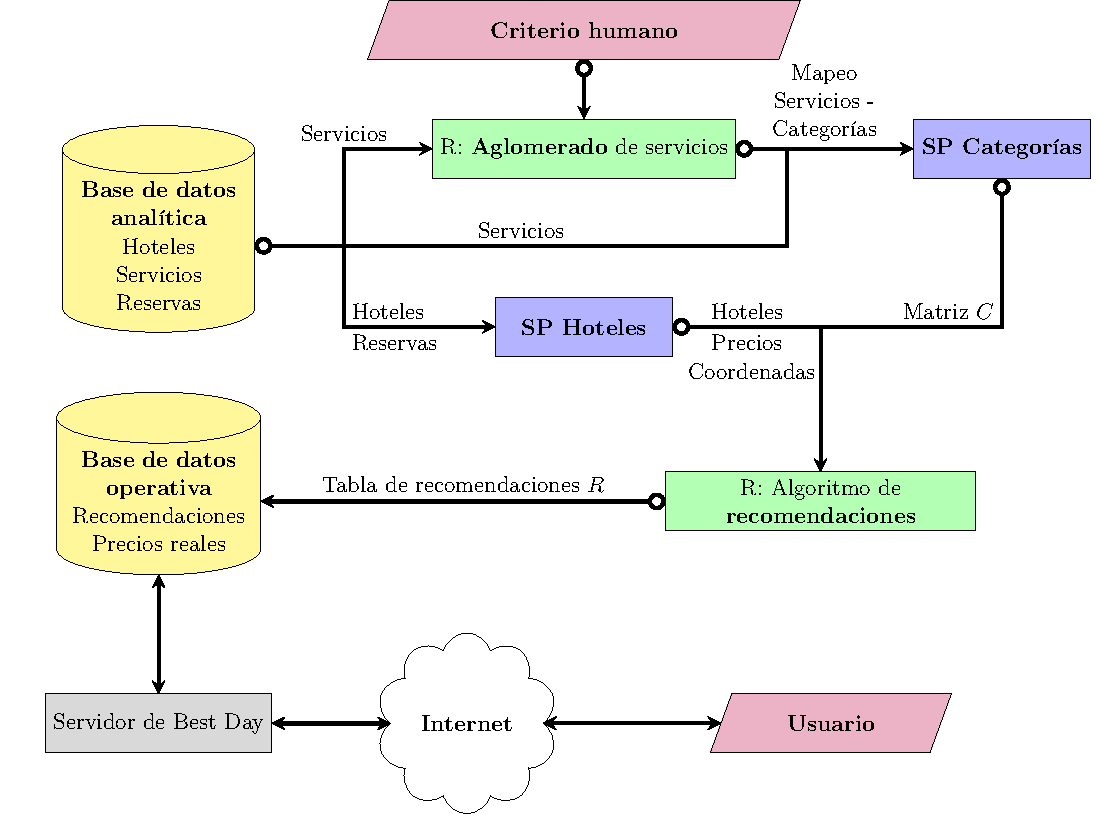
\includegraphics[width=\textwidth]{imagenes/flowchart.pdf}
\end{frame}

%%%%%%%%%%%%%%%%%%%%%%%%%%%%%%%%%%%%%%%%%%%%%%%%%
%%%%%%%%%%%%%%%%%%%%%%%%%%%%%%%%%%%%%%%%%%%%%%%%%
\section{Desempeño}

%%%%%%%%%%%%%%%%%%%%%%%%%%%%%%%%%%%%%%%%%%%%%%%%%
\begin{frame}{Desempeño de la página}
	\begin{figure}
		\centering
		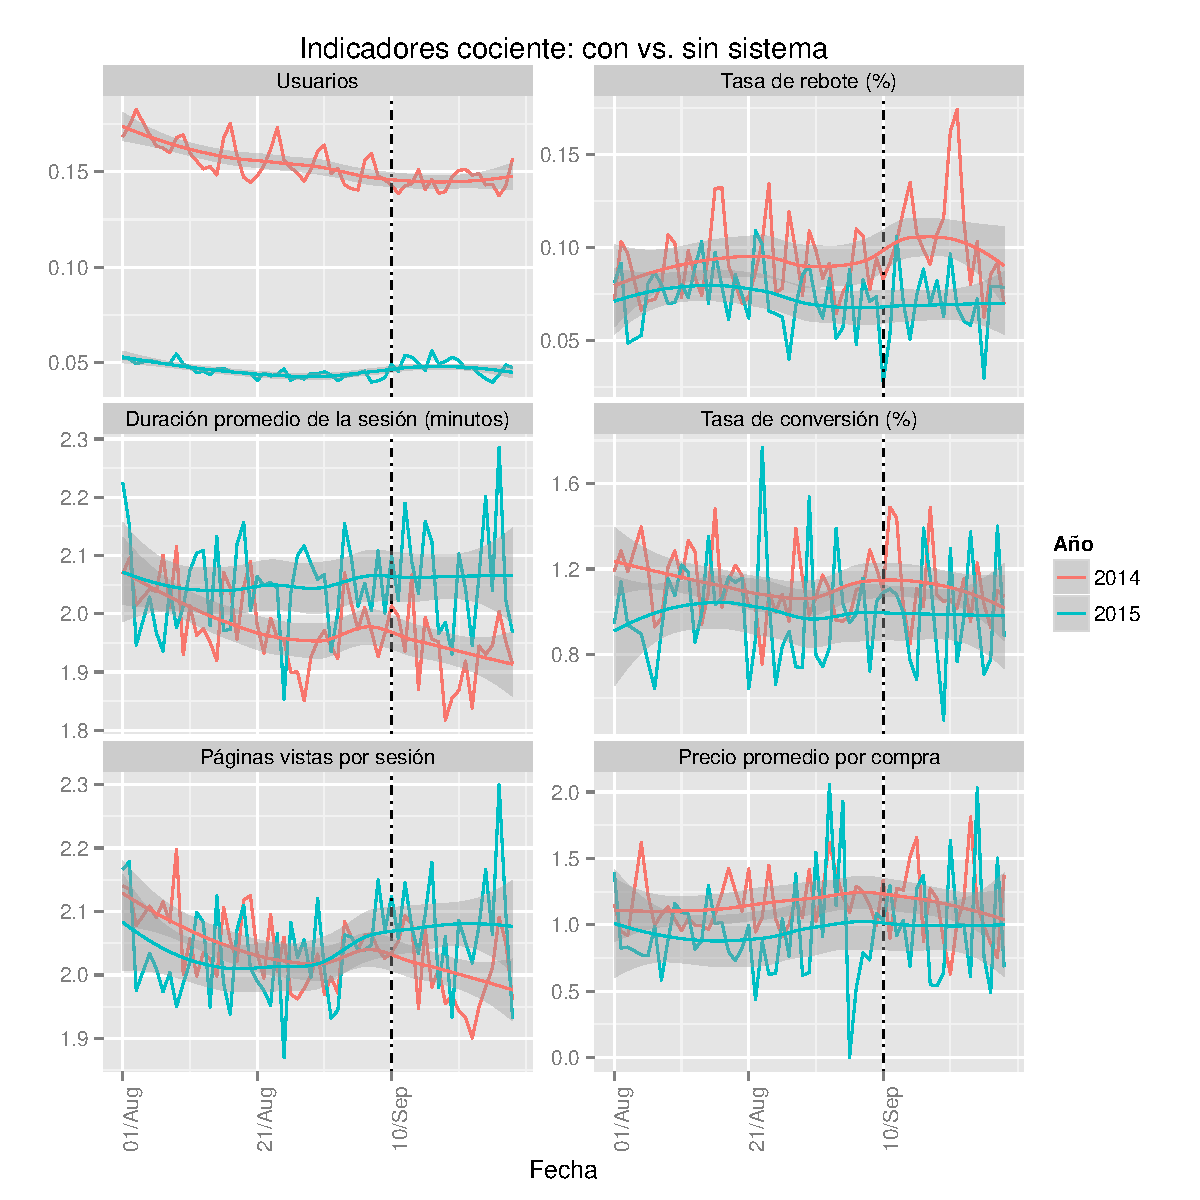
\includegraphics[width=0.7\textwidth]{imagenes/analytics_anios_y.pdf}
	\end{figure}
\end{frame}

%%%%%%%%%%%%%%%%%%%%%%%%%%%%%%%%%%%%%%%%%%%%%%%%%
\begin{frame}{Conclusiones}
	\begin{itemize}
		\item 
	\end{itemize}
\end{frame}

%%%%%%%%%%%%%%%%%%%%%%%%%%%%%%%%%%%%%%%%%%%%%%%%%
%%%%%%%%%%%%%%%%%%%%%%%%%%%%%%%%%%%%%%%%%%%%%%%%%
%%%%%%%%%%%%%%%%%%%%%%%%%%%%%%%%%%%%%%%%%%%%%%%%%
%%%%%%%%%%%%%%%%%%%%%%%%%%%%%%%%%%%%%%%%%%%%%%%%%
%%%%%%%%%%%%%%%%%%%%%%%%%%%%%%%%%%%%%%%%%%%%%%%%%
%%%%%%%%%%%%%%%%%%%%%%%%%%%%%%%%%%%%%%%%%%%%%%%%%
%%%%%%%%%%%%%%%%%%%%%%%%%%%%%%%%%%%%%%%%%%%%%%%%%
%%%%%%%%%%%%%%
%%%%%%%%%%%%%%
%%%%%%%%%%%%%%
%%%%%%%%%%%%%%

\begin{comment}
%%%%%%%%%%%%%%%%% frame %%%%%%%%%%%%%%%%%%%%%%%%%
\section{Descripci\'on del problema}

\begin{frame}{Regresi\'on log\'istica}
	\begin{itemize}[<+->] 
		\item Se modelan las probabilidades condicionales como:
		\[
			P(\mathbf{Y}=1 | \mathbf{X}=x) = p(x) = h(x^T \beta)
		\]
		\item $h$ es la funci\'on log\'istica, $h(z) = \frac{1}{1 + e^{-z}}$
		\item El ajuste es por m\'axima (log-)verosimilitud:
		\[
			\underset{\beta}{\text{maximizar \;}} \left \{ \ell(\beta) \overset{def}{=} \sum_{i=1}^n [ y_i \ln (p(x_i)) + (1 - y_i) \ln (1 - p(x_i))] \right \}
		\]
		\item Equivalentemente, minimizar la devianza:
		\[
			D(\beta) = -\frac{1}{n}\ell(\beta)
		\]
	\end{itemize}
\end{frame}

%%%%%%%%%%%%%%%%% frame %%%%%%%%%%%%%%%%%%%%%%%%%
\begin{frame}{Regresi\'on log\'istica regularizada}
	\begin{itemize}[<+->] 
		\item En general conviene regularizar
		\item El ajuste se hace resolviendo:
		\begin{align} \label{devreg}
			\underset{\beta}{\text{minimizar \;}} \left \{ DP(\beta) \overset{def}{=} D(\beta) + \lambda \sum_{j=1}^p |\beta_j| \right \}
		\end{align}
		\item $\lambda > 0$ es un par\'ametro
		\item No se regulariza $\beta_0$
		\item \textbf{Problema:} ?`C\'omo minimizar esta funci\'on num\'ericamente?
	\end{itemize}
\end{frame}

%%%%%%%%%%%%%%%%% frame %%%%%%%%%%%%%%%%%%%%%%%%%
\begin{frame}{Regresi\'on log\'istica regularizada}
	\begin{itemize}[<+->] 
		\item<1-> \textbf{Una opci\'on:} En lugar de regularizar, introducir la restricci\'on:
		\[
			\sum_{j=1}^p |\beta_j| \leq t
		\]
		\item<1-> O en su versi\'on diferenciable:
		\begin{align*}
			&\beta^a_j \geq \beta_j, \quad \beta^a_j \geq -\beta_j, \quad\text{para } j = 1, \dots, p\\
			&\sum_{j=1}^p \beta^a_j \leq t
		\end{align*}
		\item<2-> !`Se requiere agregar $p$ variables y $2p + 1$ restricciones!
		\item<3->[$\implies$] No es viable para problemas de gran escala.
	\end{itemize}
\end{frame}

%%%%%%%%%%%%%%%%% frame %%%%%%%%%%%%%%%%%%%%%%%%%
\section{M\'etodos de descenso por coordenadas}

%%%%%%%%%%%%%%%%% frame %%%%%%%%%%%%%%%%%%%%%%%%%

\begin{frame}{Repaso: M\'etodo de Newton}
	\begin{itemize}[<+->]
		\item Se quiere minimizar $f: \R^n \to \R$
		\item Equivalentemente (suponiendo convexidad), encontrar ceros de $\nabla f(x)$
		\item \textbf{Estrategia:} Minimizar el modelo cuadr\'atico de Taylor de $f$
		\begin{align*}
			q_k^N(d) \overset{def}{=} f(x_k) +  \nabla f(x_k)^Td  + \frac{1}{2} d^T \nabla^2f(x_k) d
		\end{align*}
		\item Resolviendo lo anterior se obtiene una direcci\'on de avance $d_k$
		\item Obtener un nuevo punto $x_{k+1} := x_k + \alpha_k d_k$
		\item Bajo ciertos supuestos, $x_k \to x^*$
	\end{itemize}
\end{frame}

%%%%%%%%%%%%%%%%% frame %%%%%%%%%%%%%%%%%%%%%%%%%

\begin{frame}{Adaptando Newton}
	\begin{itemize}[<+->]
		\item En este contexto hay restricciones:
		\begin{align*}
			\text{minimizar \;}  D_Q(\beta) \\
			\text{s. a \;} \sum_{j=1}^p |\beta_j| \leq t
		\end{align*}
		\item $D_Q(\beta) = $ modelo cuadr\'atico alrededor del iterando actual $\tilde{\beta}$
		\item Se vio que las restricciones no son viables
		\item \textbf{Idea:} mejor regularizar $D_Q$
		\[
			\underset{\beta}{\text{minimizar \;}} \left \{ DP_Q(\beta) = D_Q(\beta) + \lambda \sum_{j=1}^p |\beta_j| \right \}
		\]
		\item \textbf{Problema:} Es una funci\'on no diferenciable.
	\end{itemize}
\end{frame}

%%%%%%%%%%%%%%%%% frame %%%%%%%%%%%%%%%%%%%%%%%%%
\begin{frame}{Adaptando Newton}
	\begin{block}{Dato sorprendente}
		\[
			D_Q(\beta) = \frac{1}{n} \sum_{i=1}^n w_i (z_i - x_i^T \beta)^2 + C(\tilde\beta)
		\]
	\end{block}
	%\pause
	\begin{itemize}[<+->]
		\item $z_i$, $w_i$ y $C(\tilde\beta)$ s\'olo dependen de $\tilde\beta$
		\item Ajustar un modelo de MCPR en cada iteraci\'on:
		\begin{align} \label{rls}
			\underset{\beta}{\text{minimizar} \;} \left \{ \frac{1}{n} \sum_{i=1}^n w_i (z_i - x_i^T \beta)^2 + \lambda \sum_{j=1}^p |\beta_j| \right \}
		\end{align}
		\item De ah\'i el nombre \textbf{IRLS} (\textit{Iteratively Reweighted Least Squares})
	\end{itemize}
\end{frame}

%%%%%%%%%%%%%%%%% frame %%%%%%%%%%%%%%%%%%%%%%%%%
\begin{frame}{Descenso por coordenadas}
	\begin{itemize}[<+->]
		\item $DP_Q$ no es diferenciable, pero\dots
		\item \dots s\'i es predecible en las direcciones $e_1, \dots, e_p$
		\item Usar el enfoque de descenso por coordenadas:
		\begin{align} \label{cd}
			\underset{\beta_j}{\text{minimizar} \;} \left \{ \frac{1}{n} \sum_{i=1}^n w_i (z_i - x_i^T \beta)^2 + \lambda \sum_{j=1}^p |\beta_j| \right \}
		\end{align}
		\item \textbf{Resultado importante:} Existe una f\'ormula cerrada para la soluci\'on de (\ref{cd})
	\end{itemize}
\end{frame}

%%%%%%%%%%%%%%%%% frame %%%%%%%%%%%%%%%%%%%%%%%%%
\begin{frame}{Descenso por coordenadas}
	\begin{block}{F\'ormula cerrada}
		\begin{enumerate}[(i)]
			\item $\tilde\beta_0 \leftarrow \sum_{i=1}^n w_i y_i$
			\item $\tilde\beta_j \leftarrow S(\sum_{i=1}^n w_i x_{ij} r_i + \tilde\beta_j, \lambda)$
		\end{enumerate}
	\end{block}
	%\pause
	\begin{itemize}
		\item $r_i = y_i - x_i^T \tilde\beta = y_i - \hat{y}_i$ es el residual actual.
		\item $S: \R \times (\R^+ \cup \{0\}) \to \R$ es el \emph{operador de umbral suave}:
			\[
				S(z, \gamma) = \text{signo}(z) (|z| - \gamma)_+ = \left \{
				\begin{array}{ll}
					z - \gamma & \text{si } z > 0 \text{ y } \gamma < |z| \\
					z + \gamma & \text{si } z < 0 \text{ y } \gamma < |z| \\
					0                  & \text{si } \gamma \geq |z|
				\end{array}
				\right.
			\]
		%\pause	
		\item Ejemplo ilustrativo...
	\end{itemize}
\end{frame}

%%%%%%%%%%%%%%%%% frame %%%%%%%%%%%%%%%%%%%%%%%%%
\begin{frame}{Algoritmos}
	\begin{itemize}
		\item[(1)] \textbf{M\'inimos Cuadrados Ponderados:}
		\begin{itemize}
			\item Asignar $\beta_0$ con la f\'ormula (I)
			\item Repetir hasta satisfacer el criterio de paro:\\
			\begin{itemize}
				\item[1.-] Actualizar los coeficientes uno por uno con la f\'ormula (II)
			\end{itemize}
		\end{itemize}
		\vspace{20pt}
		\item[(2)] \textbf{IRLS (para regresi\'on log\'istica):}
		\begin{itemize}
			\item Repetir hasta satisfacer el criterio de paro:
			\begin{itemize}
				\item[1.-] Calcular $w_i$ y $z_i$
				\item[2.-] Correr el algoritmo (1)
			\end{itemize}
		\end{itemize}
	\end{itemize}
\end{frame}

%%%%%%%%%%%%%%%%% frame %%%%%%%%%%%%%%%%%%%%%%%%%

%\begin{frame}{Propiedades de IRLS}
%	\begin{itemize}[<+->]
%		\item \textbf{Ventajas:}
%		\begin{itemize}[<+->]
%			\item Las iteraciones son muy r\'apidas
%			\item Es muy r\'apido y sorprendentemente robusto
%			\item Est\'a implementado en R
%		\end{itemize}
%		\item \textbf{Desventajas:}
%		\begin{itemize}[<+->]
%			\item Es dif\'icil reproducir una versi\'on aceptable
%			\item Est\'a implementado exclusivamente en R
%		\end{itemize}
%	\end{itemize}
%\end{frame}

%%%%%%%%%%%%%%%%% frame %%%%%%%%%%%%%%%%%%%%%%%%%
\section{M\'etodos cuasi-Newton}

\begin{frame}{Repaso: M\'etodos cuasi-Newton}
	\begin{itemize}[<+->] 
		\item Sustituir $\nabla^2f(x_k)$ con una matriz sim\'etrica $B_k$
		\item Minimizar el modelo cuadr\'atico aproximado para obtener $d_k$:
		\begin{align*}
			q^C_{k}(d) \overset{def}{=} \frac{1}{2} d^T B_{k} d + \nabla f(x_{k})^T d + f(x_{k})
		\end{align*}
		\item Soluci\'on: $d_k = -B_k^{-1}  \nabla f(x_{k})$.
		\item Alternativa: obtener directamente $H_k = B_k^{-1}$.
		\item Actualizaci\'on BFGS:
		\begin{align*}
			&H_{k+1} = (I - \rho_k s_k y_k^T) H_k (I - \rho_k y_k s_k^T) + \rho_k s_k s_k^T\\
			&\text{donde } s_k = x_{k+1} - x_k;\; y_k = \nabla f(x_{k+1}) - \nabla f(x_k);\; \rho_k = \frac{1}{y_k^T s_k}
		\end{align*}
		\item Variante para gran escala: L-BFGS.
	\end{itemize}
\end{frame}

%%%%%%%%%%%%%%%%% frame %%%%%%%%%%%%%%%%%%%%%%%%%

\begin{frame}{Motivaci\'on de OWL-QN}
	\begin{itemize}[<+->]
		\item Se quiere...
		\begin{itemize}
			\item[1.-] Evitar usar restricciones
			\item[2.-] Aprovechar la informaci\'on de segundo orden
		\end{itemize}
		\item \textbf{Problema:} $DP(\beta)$ no es diferenciable
		\item Propuesta de OWL-QN: Generalizar L-BFGS
		\item En vez del gradiente usar el pseudo-gradiente $\diamond f(x)$:
		\[
			\diamond_i f(x) = \left \{
			\begin{array}{ll}
				\partial^-_i f(x) & \text{si } \partial^-_i f(x) > 0\\
				\partial^+_i f(x) & \text{si } \partial^+_i f(x) < 0\\
				0                       & \text{en otro caso}
			\end{array} \right .
		\]
	\end{itemize}
\end{frame}

%%%%%%%%%%%%%%%%% frame %%%%%%%%%%%%%%%%%%%%%%%%%

% IMAGEN DE PSEUDOGRADIENTE % CREO QUE NO ES NECESARIA

%%%%%%%%%%%%%%%%% frame %%%%%%%%%%%%%%%%%%%%%%%%%

\begin{frame}{Descripci\'on del algoritmo}
	\begin{itemize}[<+->]
		\item Identificar el espacio en el que queremos buscar,
		\[
			\Omega_\xi = \{ \beta \in \R^{p+1} \; | \; \pi(\beta;\xi) = \beta \}
		\]
		\item Construir $DP_\xi(\beta) \in \mathcal{C}^1$ que sea igual a $DP(\beta)$ en $\Omega_\xi$
		\item Proyectar $-\nabla DP_\xi(\beta^{(k)})$ sobre $\text{gen}\; \Omega_\xi$:
		\[
			v_k = \mathbb{P}(-\nabla DP_\xi(\beta^{(k)}))
		\]
		\item Elecci\'on particular de $\xi \implies v_k = -\diamond DP(\beta^{(k)})$
		\item Obtener $H_k$ mediante la f\'ormula L-BFGS
		\item Avanzar en la direcci\'on $p^{(k)} = \pi(H_kv_k; v_k)$
		\item Finalmente, b\'usqueda de l\'inea restringida a $\Omega_\xi$
	\end{itemize}
\end{frame}

%%%%%%%%%%%%%%%%% frame %%%%%%%%%%%%%%%%%%%%%%%%%

% DIBUJO DE LO QUE HACE OWL-QN?

%%%%%%%%%%%%%%%%% frame %%%%%%%%%%%%%%%%%%%%%%%%%

%\begin{frame}{Propiedades de OWL-QN}
%	\begin{itemize}[<+->]
%		\item \textbf{Ventajas:}
%		\begin{itemize}[<+->]
%			\item Utiliza informaci\'on de curvatura de bajo costo
%			\item Es escalable a muchas variables
%			\item Es razonablemente r\'apido
%		\end{itemize}
%		\item \textbf{Desventajas:}
%		\begin{itemize}[<+->]
%			\item Las trayectorias son inestables y poco suaves
%			\item Implementaci\'on poco amigable (consola)
%			\item Poco flexible con el tipo de datos que admite
%		\end{itemize}
%	\end{itemize}
%\end{frame}

%%%%%%%%%%%%%%%%% frame %%%%%%%%%%%%%%%%%%%%%%%%%
\section{Pruebas num\'ericas}

\begin{frame}{Ejemplos simulados}
	\begin{itemize}[<+->]
		\item Variables simuladas + ruido $\to$ respuesta
		\item Regresi\'on log\'istica $n = 3,000$, $p = 50$ (regularizaci\'on recomendada)
		\item Regresi\'on log\'istica $n = 100$, $p = 200$ (regularizaci\'on forzosa)
		\vspace{10pt}
		%\pause
		\begin{table}[h]
			\centering
			\begin{tabular}{|l|l|c|c|c|}
			\hline
			n 		& p 		& glmnet 		& nuestro 				& OWL-QN\\
			\hline
			3000		& 50 		& 0.997$\star$	&	68.965			& 28.682	\\
			100		& 200	& 0.022$\star$	&	10.502			& 3.368	\\
			\hline
			\end{tabular}
		\end{table}
		\vspace{10pt}
		\item \texttt{glmnet} parece ser superior
		\item OWL-QN es mejor que nuestra versi\'on $\to$ c\'odigo optimizado
	\end{itemize}
\end{frame}


%%%%%%%%%%%%%%%%% frame %%%%%%%%%%%%%%%%%%%%%%%%%

\begin{frame}{C\'ancer de mama}
	\begin{itemize}[<+->]
		\item Diagnosticar c\'ancer de mama es dif\'icil
		\item Depende de la habilidad del doctor
		\item \textbf{Alternativa:} FNA (\emph{fine needle aspirate})
		\item Prueba poco invasiva + \emph{machine learning}
		\item 569 casos de entrenamiento y 30 variables
		\vspace{20pt}
		\begin{table}[h]
			\centering
			\begin{tabular}{|c|c|}
			\hline
			Algoritmo 		& Tiempo de ejecuci\'on (seg)\\
			\hline
			\emph{glmnet}		& 0.047$\star$ 	\\
			OWL-QN		& 3.86	\\
			nuestro		& 11.152	\\
			\hline
			\end{tabular}
		\end{table}
	\end{itemize}
\end{frame}

%%%%%%%%%%%%%%%%% frame %%%%%%%%%%%%%%%%%%%%%%%%%

\begin{frame}{C\'ancer de mama}
	\begin{figure}
		\begin{minipage}{0.3\textwidth} % each column can also be its own environment
%			\includegraphics[width=\textwidth]{./graficas/cancer_glmnet.pdf}
%			\caption{\texttt{glmnet}}
		\end{minipage}
		\begin{minipage}{0.3\textwidth} 
%			\includegraphics[width=\textwidth]{./graficas/cancer_my.pdf}
%			\caption{DC propio}
		\end{minipage}
		\begin{minipage}{0.3\textwidth} 
%			\includegraphics[width=\textwidth]{./graficas/cancer_owl.pdf}
%			\caption{OWL-QN}
		\end{minipage}
	\end{figure}
\end{frame}

%%%%%%%%%%%%%%%%% frame %%%%%%%%%%%%%%%%%%%%%%%%%

\begin{frame}{\emph{Spam}}
	\begin{itemize}[<+->]
		\item Filtro autom\'atico de \emph{spam}
		\item Una persona califica una base de mails
		\item Variables: frecuencia de palabras o de s\'imbolos
		\item 3,067 casos de entrenamiento y 57 variables
		\vspace{20pt}
		\begin{table}[h]
			\centering
			\begin{tabular}{|c|c|}
			\hline
			Algoritmo 		& Tiempo de ejecuci\'on (seg)\\
			\hline
			\emph{glmnet}		& 1.654$\star$ 	\\
			OWL-QN		& 19.291	\\
			nuestro		& $\dagger$ (75.563)	\\
			\hline
			\end{tabular}
		\end{table}
	\end{itemize}
\end{frame}

%%%%%%%%%%%%%%%%% frame %%%%%%%%%%%%%%%%%%%%%%%%%

%%%%%%%%%%%%%%%%% frame %%%%%%%%%%%%%%%%%%%%%%%%%
\section{Conclusiones}

\begin{frame}{Resumen de caracter\'isticas}
	\begin{table}[h]
		\centering
		\begin{tabular}{|l|l|l|}
		\hline
		&	\texttt{glmnet} & OWL-QN\\
		\hline
		Info. de $2^o$ orden & \cmark (outer) & \cmark (cuasi-Newton)\\
		\hline
		Escalable & \cmark & \cmark\\
		\hline
		R\'apido & \cmark & OK \\
		\hline
		Robusto (corre bien) & \cmark & \xmark \;($\lambda \to \infty$, b. de l\'inea) \\
		\hline
		Estable (trayectorias) & \cmark & \xmark \\
		\hline
		F\'acil de usar / flexible & \cmark \;(\texttt{R}) & \xmark \;(consola)\\
		\hline
		F\'acil de implementar (bien) & \xmark & N/A \\
		\hline
		Disponibilidad (otros paq.) & \xmark & \xmark \\
		\hline
		\end{tabular}
	\end{table}
\end{frame}

%%%%%%%%%%%%%%%%% frame %%%%%%%%%%%%%%%%%%%%%%%%%

\begin{frame}{Conclusiones}
	\begin{itemize}[<+->] \itemsep4ex
		\item[(1)] \textbf{Regularizar} es fundamental en \emph{machine learning}
		\item[(2)] Descenso por coordenadas (\texttt{glmnet}) \textbf{domina} a OWL-QN
		\item[(3)] \textbf{No es f\'acil} implementar una versi\'on r\'apida y robusta
		\item[(4)] La \textbf{documentaci\'on} deja mucho que desear
		\item[(5)] \textbf{Falta} para que se incluya en paquetes comerciales
	\end{itemize}
\end{frame}

%%%%%%%%%%%%%%%%%%%%% Bibliografia %%%%%%%%%%%%%%%%%%%%%%%%
\begin{frame}{Bibliograf\'ia}
    \begin{thebibliography}{1}
    
    \bibitem{owlqn}
	Andrew, Galen y Gao, Jianfeng. (2007). Scalable Training of $L_1$-Regularized Log-Linear Models.  \emph{International Conference on Machine Learning.} pp. 33-40.
	
    \bibitem{convex}
        Boyd, Stephen y Lieven Vandenberghe. (2009). \emph{Convex Optimization}, Cambridge University Press.
    
    \bibitem{clarke}
        Clarke, Frank H. (1990). \emph{Optimization and Nonsmooth Analysis}, SIAM.
    
    \bibitem{glmnet}
        Friedman, Jerome; Hastie Trevor y Tibshirani Robert. (2010). Regularization Paths for Generalized Linear Models via Coordinate Descent. \emph{Journal of Statistical Software}.
    \end{thebibliography}
\end{frame}

\begin{frame}{Bibliograf\'ia}
    \begin{thebibliography}{1}
    
    \bibitem{elements}
        Friedman, Jerome; Hastie Trevor y Tibshirani Robert. (2008). \emph{The Elements of Statistical Learning. Data Mining, Inference and Prediction. Second Edition}, Springer, 2008.
    
    \bibitem{cancer}
	Mangasarian, Olvi L. et al. (1995). Breast Cancer Diagnosis and Prognosis via Linear Programming. \emph{Operations Research}. vol. 43, no. 4, pp. 570-577.
		
    \bibitem{nocedal}
    	Nocedal, Jorge y Wright, Stephen J. (2006). \emph{Numerical Optimization. Second Edition}, Springer.
    
    \end{thebibliography}
\end{frame}

%%%%%%%%%%%%%%%%% frame %%%%%%%%%%%%%%%%%%%%%%%%%
\begin{frame}{Fin de la exposici\'on}
    \only<2>{
    	\begin{center}
    	    \Huge
    		Preguntas
    	\end{center}
    }
\end{frame}


\end{comment}





\end{document} 

















